\chapter{Set-up of experiment}
Some equipment and materials are needed to perform the experiments. These are shown in the fig. \ref{fig:setup} and listed again below.
%
\begin{figure}[H]
	\begin{center}
		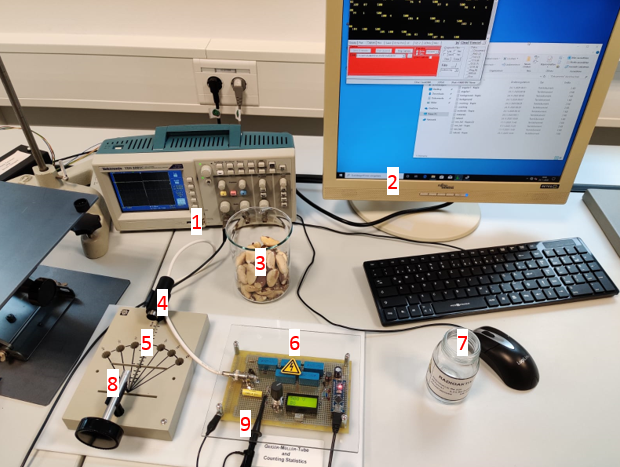
\includegraphics[width=14cm]{setup.png}
		\caption{Equipment and material required for the experiments.}  
		\label{fig:setup} 
	\end{center}
\end{figure}
%
\begin{enumerate}
	\item Oscilloscope
	\item Computer with the software RealTerm
	\item Beaker with Brazil nuts
	\item Geiger-Müller tube
	\item Mounting plate
	\item Circuit board
	\item Protective container
	\item Radioactive source ($^{226}$Ra, 3.3 kBq)
	\item Oscilloscope probe with ground clip
\end{enumerate}
%
A better view of the circuit board will give fig. \ref{fig:circuit_board}. Again, the components are listed below.
%
\begin{figure}[H]
	\begin{center}
		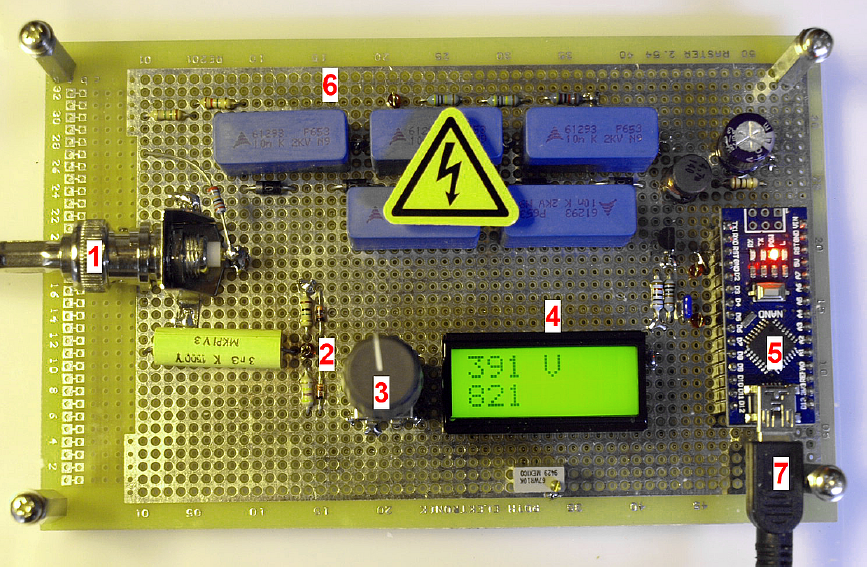
\includegraphics[width=14cm]{circuit_board.png}
		\caption{Circuit board in greater detail. (Source: A. Doerr, Geiger-Mueller Tube and Counting Statistics, page 5)}  
		\label{fig:circuit_board} 
	\end{center}
\end{figure}
%
\begin{enumerate}
	\item BNC connector
	\item Testpoint
	\item Potentiometer
	\item LCD
	\item Arduino nano
	\item Boost converter
	\item USB port
\end{enumerate}
%
To begin with the experiments, the computer is started first. When the computer is ready, the program RealTerm is being started. The following settings are made:
\begin{itemize}
	\item In the \texttt{Port} tab, 9600 is selected for \texttt{Baud}.
	\item The microcontroller is connected with the computer and the assigned COM number is selected under \texttt{Port}.
	\item On the \texttt{Display} tab, \texttt{Ascii} and \texttt{new Line mode} are checked, \texttt{Direct capture} is un-checked.
\end{itemize}
%
The data is now continuously sent by the microcontroller. The data is displayed on the screen. A text file is created in which the data is written and saved. Three columns are displayed. The first column contains the number of the measurement, the second the counts per 10 s and the third the present voltage $U_{GMT}$.\\
Now the oscilloscope is switched on. The probe tip is connected to the test point. The ground clip is attached to the housing of the circuit board. The display is adjusted so that a single radioactive event fills the screen when the trigger is set correctly.\\
Now the setup is completed and the experiments can be started.
